\documentclass[11pt,a4paper]{article}

\usepackage[T1]{fontenc}
\usepackage[utf8]{inputenc}
\usepackage[margin=1in]{geometry}
\usepackage{amsmath,amssymb}
\usepackage{booktabs}
\usepackage{array}
\usepackage{enumitem}
\usepackage{graphicx}
\usepackage{float}
\usepackage{listings}
\usepackage[hidelinks]{hyperref}
\usepackage{caption}

\captionsetup{font=small,labelfont=bf}
\captionsetup[table]{skip=6pt}
\captionsetup[figure]{skip=8pt}

\lstset{
  basicstyle=\ttfamily\small,
  frame=none,
  xleftmargin=2em,
  breaklines=true,
  columns=fullflexible,
  keepspaces=true,
  showstringspaces=false,
  aboveskip=10pt,
  belowskip=10pt
}

\setlength{\parskip}{0pt}
\setlength{\parindent}{1.5em}

% Design-decision block: plain indented text, italic run-in labels
\newcommand{\designnote}[3]{%
  \par\vspace{7pt}
  \begin{list}{}{%
    \setlength{\leftmargin}{2em}\setlength{\rightmargin}{1em}%
    \setlength{\labelwidth}{0pt}\setlength{\labelsep}{0pt}%
    \setlength{\itemsep}{2pt}\setlength{\topsep}{0pt}%
    \setlength{\parsep}{0pt}}
    \item[]\textit{Previously.}~#1
    \item[]\textit{Issue.}~#2
    \item[]\textit{Revised.}~#3
  \end{list}
  \par\vspace{7pt}
}

\title{Borrower Health Index and Recovery Estimation\\
\large Reconstructing a Credit Bureau Score from Repayment Behaviour}
\author{}
\date{}

\begin{document}
\maketitle

\section{Introduction}

The Home Credit Default Risk dataset includes \texttt{EXT\_SOURCE\_\allowbreak 1/2/3}: proprietary
external credit scores derived from credit bureau records spanning a borrower's complete
history across all lenders. These features rank among the strongest predictors available
in the dataset.

A bureau score is comprehensive in breadth. A lender's own installment records are
narrower in scope but substantially denser in temporal granularity, capturing exact
payment timing, partial settlement behaviour, and prioritisation between competing
obligations.

This project quantifies the trade-off between these information sets:

\begin{quote}
\textit{How much of a commercial bureau score can be reconstructed from repayment
behaviour alone?}
\end{quote}

The pipeline is constructed as an internal, behaviour-only credit score and evaluated
against Home Credit's external score on identical held-out borrowers.

\designnote{External scores treated as ordinary input features, entering the model
alongside behavioural features.}
{With the strongest available predictor supplied directly as an input, the pipeline's own
contribution could not be isolated. Any performance figure would conflate signal
extracted from repayment behaviour with signal supplied by the bureau, leaving the stated
question unanswerable.}
{External scores held out as an independent benchmark and scored separately, so the
behavioural pipeline is measured against them rather than through them. An ablation
quantifying their standalone contribution is reported in Section~6.1.}

\section{Data}

\begin{table}[H]
\centering
\caption{Data sources and their contribution to the modelling panel}
\begin{tabular}{p{0.30\textwidth}p{0.58\textwidth}}
\toprule
\textbf{Source} & \textbf{Contribution} \\
\midrule
\texttt{installments\_\allowbreak payments.csv} & Per-installment repayment behaviour: amount
due, amount paid, payment timing \\
\addlinespace
\texttt{application\_train.csv} & Borrower context: income, credit exposure, employment
tenure, \texttt{EXT\_SOURCE\_*}, \texttt{TARGET} \\
\bottomrule
\end{tabular}
\end{table}

\vspace{6pt}

16,632 borrowers loaded; 12,991 retained following the baseline estimation window; 1,673
reach final evaluation, of which 138 are eventual defaulters.

\designnote{Sample of 3,000 borrowers, with only \texttt{TARGET} drawn from the
application table.}
{The sample yielded too few defaulters for stable interval estimation, and the
application table --- already being read --- was contributing a single label column while
its borrower-context fields were discarded. Income, credit exposure and employment tenure
were available at no additional cost and were not being used.}
{Sample increased to 20,000 borrowers, and ten borrower-context features derived from the
application table, including credit-to-income and annuity-to-income ratios, employment
tenure and regional population density.}

\designnote{Loader falling back to a synthetic panel when the source files were absent.}
{A silent fallback permits results to be produced from generated data without any
indication in the output, and any figure so produced is indistinguishable from a genuine
one downstream.}
{The loader raises on missing source files. No synthetic path exists in the pipeline.}

\designnote{Baseline estimation window of three months.}
{Borrowers average approximately six usable observation periods. Reserving three for
baseline estimation left too few for trajectory construction, and the loss compounded
with the lagging requirement, which consumes a further period.}
{Window reduced to two periods, retaining sufficient data for stable stress estimation
while releasing an additional period to the modelling panel.}

\paragraph{Temporal representation.} Home Credit provides day-offsets rather than
calendar dates. Monthly periods are approximated as 30.44-day buckets measured from each
borrower's first observed installment. The anchoring choice is material and is discussed
in Section~\ref{sec:lagging}.

\section{Feature Construction}

The behavioural score derives exclusively from repayment records, placing the burden of
representation on feature construction.

\subsection{Signed payment timing}

\texttt{PAYMENT\_\allowbreak WINDOW\_\allowbreak DAYS} preserves sign, with negative values indicating early
settlement.

\designnote{Payment timing encoded as \texttt{DAYS\_PAST\_DUE}, clipped at zero.}
{Clipping discards the distinction between borrowers settling ahead of schedule and those
settling precisely on time. These are behaviourally distinct populations with different
risk profiles, collapsed into a single value of zero.}
{Signed timing retained as a separate feature, with the clipped variant kept alongside it
for the ``how overdue'' signal specifically.}

\texttt{PAY\_WINDOW\_STD\_3M} captures dispersion in payment timing independently of its
central tendency.

\designnote{Rolling mean of payment timing (\texttt{PAY\_\allowbreak WINDOW\_\allowbreak ROLLING\_3M}) and its
deviation from the current value (\texttt{TIMING\_DRIFT}).}
{A mean cannot distinguish a borrower consistently five days late, reflecting a stable
payday cycle, from one alternating between ten days early and fifteen days late,
reflecting irregular income. Both produce identical rolling means.}
{Rolling standard deviation added, capturing dispersion separately from central tendency.}

\subsection{Payment fragmentation}

The installment data records multiple payment rows against a single due installment,
representing an obligation settled across several transactions.

\designnote{Each payment row treated as an independent observation.}
{A EUR 400 obligation settled as three transactions of EUR 150, EUR 150 and EUR 100 was
indistinguishable from a single EUR 400 settlement. The obligation is met in full and on
schedule in both cases, but the fragmented case indicates a liquidity constraint.}
{\texttt{N\_PAYMENT\_SPLITS} counts payment rows per due installment;
\texttt{SPLIT\_\allowbreak PAYMENT\_\allowbreak RATE\_3M} tracks the rolling share of obligations requiring
multiple transactions.}

This signal exists only in transaction-level records held by the originating lender and
is not observable at bureau level.

\subsection{Obligation prioritisation}

Borrowers holding multiple obligations do not default uniformly. Under liquidity pressure
they triage, protecting certain obligations while permitting others to lapse. A Gaussian
mixture model over obligation-level features infers which obligations are prioritised
(Section~\ref{sec:priority}). \texttt{PRIORITY\_\allowbreak SPREAD} measures divergence in inferred
priority within a borrower-month, and \texttt{SELECTIVE\_\allowbreak FAILURE} measures the
corresponding divergence in realised payment performance between the highest- and
lowest-priority obligations.

\subsection{Trend features}

\texttt{PAYMENT\_\allowbreak RATIO\_\allowbreak TREND\_3M} and \texttt{DPD\_TREND\_3M} encode direction of
movement rather than level, constructed entirely from lagged observations.

\designnote{Direction inferred implicitly from the difference between a current value and
its rolling mean.}
{A deviation from a rolling mean conflates two distinct situations: a single anomalous
period against a stable history, and a sustained trend that the rolling window has partly
absorbed. The two carry different risk implications and were not separable.}
{Explicit trend features differencing lagged values across a fixed interval, so
directional movement is represented independently of deviation from a moving average.}

\section{Methodology}

\subsection{Framing}

Conventional credit modelling treats default as binary classification over a borrower
snapshot. This project adopts a framing drawn from industrial reliability engineering, in
which assets are assigned a continuously measured condition and Remaining Useful Life
models forecast the degradation trajectory to enable intervention prior to failure.

\begin{table}[H]
\centering
\caption{Correspondence between industrial asset monitoring and consumer credit}
\begin{tabular}{ll}
\toprule
\textbf{Industrial asset monitoring} & \textbf{Consumer credit} \\
\midrule
Measured asset condition & Health Score $H(t)$ \\
Degradation rate & Forecast $\Delta H(t{+}1)$ \\
Remaining Useful Life & Time to default \\
Maintenance scheduling & Collections prioritisation \\
Cost of unplanned failure & Unrecovered balance \\
\bottomrule
\end{tabular}
\end{table}

\designnote{Default modelled as binary classification over a borrower snapshot.}
{A binary formulation produces a decision but no timing. It cannot express how far a
borrower is from the threshold, in which direction they are moving, or how much time
remains before intervention becomes necessary --- all of which are operationally
required for collections prioritisation.}
{Continuous health score with an explicit degradation trajectory, yielding alert timing,
monitoring tier assignment and expected recovery alongside the binary decision.}

\subsection{Baseline stress estimation}

Each borrower is assigned a latent financial stress parameter $\theta_i$, with
obligation-level priority $p_{ij}$, under the generative model
\begin{align}
r_{ij} &= 1 - \theta_i(1 - p_{ij}) + \varepsilon, \qquad \varepsilon \sim \mathcal{N}(0,\sigma^2) \\
\theta_i &\sim \mathrm{TruncNormal}(0, \tau_\theta^2) \ \text{on} \ [0,\infty) \\
p_{ij} &\sim \mathrm{TruncNormal}(0.5, \tau_p^2) \ \text{on} \ [0,1]
\end{align}
where $r_{ij}$ is the realised payment ratio. A borrower under stress underpays, except
on obligations treated as high priority. Both conditional distributions are
linear-Gaussian given the other parameter, so each Gibbs update reduces to a closed-form
truncated-normal draw. The sampler runs 300 iterations with 100 discarded to burn-in.

\designnote{$\theta_i$ estimated over each borrower's complete observation history.}
{An observation at month 5 carried a parameter informed by months 6 onward. Because
$\theta_i$ appears static, this transmitted future information through a variable that
does not visibly vary. This defect alone accounted for a substantial share of an
implausible reported $R^2 = 0.985$.}
{$\theta_i$ estimated exclusively from each borrower's initial observation window, then
frozen. Window observations are excluded from the modelling panel, so no row is scored
using a parameter it helped estimate.}
\begin{figure}[H]
\centering
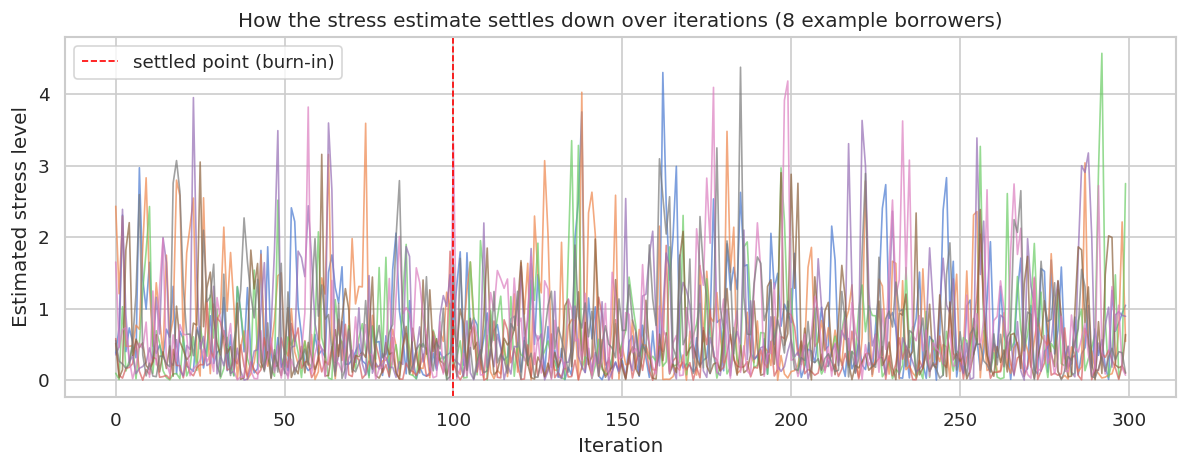
\includegraphics[width=0.88\textwidth]{figures/fig1_gibbs_traces.png}
\caption{Gibbs sampler traces for eight randomly selected borrowers. The vertical rule marks
the burn-in cutoff at 100 iterations; chains are stationary well before this point.
Posterior means over the retained draws form the frozen $\theta_i$ estimates.}
\label{fig:gibbs}
\end{figure}


\subsection{Obligation prioritisation model}
\label{sec:priority}

\subsubsection*{Why a mixture model}

When a borrower holds several concurrent obligations, the quantity of interest is not
observable: no field records which loan the borrower is choosing to protect. What is
observable is the outcome of that choice --- some obligations settle promptly and in
full, others lapse, within the same borrower and the same month.

This is a latent class problem. The population of obligations is assumed to arise from
two unobserved regimes, one prioritised and one deprioritised, and the task is to recover
regime membership from observed settlement behaviour. A Gaussian mixture is the natural
estimator for this structure: it models the observed distribution as arising from
unobserved components, and returns a posterior probability of membership rather than a
hard assignment.

The soft assignment matters downstream. \texttt{PRIORITY\_\allowbreak SPREAD} measures
the divergence in inferred priority \emph{within} a borrower-month, which requires a
continuous membership score; a hard clustering would collapse it to a binary indicator
and discard the degree of divergence, which is precisely the stress signal of interest.

Two components were specified rather than selected by information criterion. The
construct being estimated is binary by definition --- an obligation is either being
protected or it is not --- so component count is fixed by the modelling question rather
than by fit statistics.

\subsubsection*{Specification}

A two-component Gaussian mixture over eleven obligation-level features. The reliable
component is identified by lowest mean days-past-due.

\designnote{Five features: installment amount, days past due, signed payment window,
payment count, and baseline stress.}
{The model was assigning priority from a narrow view of each obligation, with no access
to the recent behavioural context already engineered elsewhere in the pipeline. Priority
inference was consequently coarser than the information available.}
{Expanded to eleven features, adding lagged payment ratio, lagged and rolling maximum
days-past-due, payment fragmentation, and timing dispersion --- giving the prioritisation
model the same behavioural depth as the forecasting stage.}

\designnote{Component identified by fixed positional index into the fitted means array.}
{The index silently referred to a different feature whenever the feature list changed,
selecting the wrong component without raising an error.}
{Component resolved by feature name, so the lookup remains correct under feature list
modification.}

\designnote{Priority aggregated as a within-month mean
(\texttt{AVG\_PRIORITY\_SCORE}), recomputed independently each period.}
{A memoryless per-period average discards continuity and admits period-to-period noise
directly into the health scorecard.}
{\texttt{CURRENT\_PRIORITY} maintained as an exponentially-weighted running estimate, so
each period's mixture output refines a carried-forward prior rather than replacing it.}

The mixture model is fit exclusively on training borrowers; test observations are scored
by transform without refitting.

\subsection{Health scorecard}

The health score is a logistic regression estimating probability of good standing,
consistent with standard credit scorecard construction and yielding directly
interpretable per-feature coefficients.

\designnote{A second Gaussian mixture clustering borrower-months into latent health
regimes, with the health score derived from component posterior probabilities.}
{Clustering is unsupervised, whereas a credit score is a supervised risk estimate. The
posterior probabilities additionally concentrated at the boundaries of $[0,1]$, producing
a bimodal distribution that destabilised downstream trajectory forecasting.}
{Logistic regression against realised outcome, producing a smooth score with signed,
interpretable coefficients.}

\designnote{Fixed default regularisation.}
{Four correlated delinquency features assumed large opposing coefficients, causing
\texttt{MAX\_DPD} to acquire a positive sign --- implying that greater delinquency
implies improved health. A multicollinearity artifact rather than a substantive effect.}
{Regularisation strength selected by five-fold cross-validation, shrinking correlated
coefficients toward one another and restoring coefficient coherence.}

\designnote{Temporal smoothing by centered median window over $(t{-}1, t, t{+}1)$.}
{A centered window smooths period $t$ using period $t{+}1$, transmitting forward
information into a feature intended for causal use.}
{Trailing median window over $(t{-}2, t{-}1, t)$.}
\begin{figure}[H]
\centering
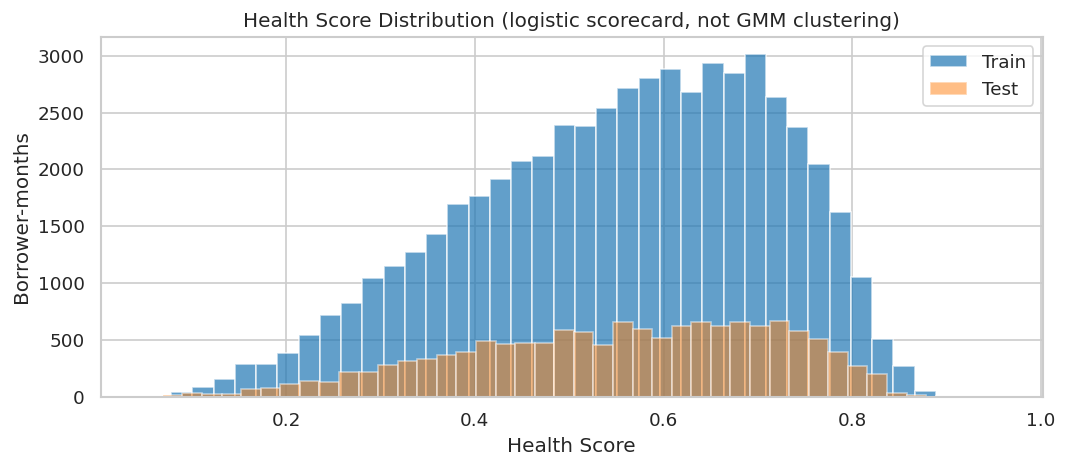
\includegraphics[width=0.80\textwidth]{figures/fig2_health_distribution.png}
\caption{Distribution of the smoothed health score across borrower-months, train and test.
The distribution is unimodal and continuous, in contrast to the boundary concentration
produced by the superseded mixture-model formulation.}
\label{fig:healthdist}
\end{figure}


\subsection{Trajectory forecasting}

The forecast target is $\Delta\,\mathrm{logit}(H)$ rather than $\Delta H$.

\designnote{Forecasting $\Delta H$ directly in probability space, with the result clipped
to $[0,1]$ after each step.}
{Since $H$ is bounded, an additive step carries position-dependent meaning: a movement of
0.05 is routine at $H = 0.50$ and infeasible at $H = 0.02$. Under recursive simulation,
clipping caused trajectories to saturate at the boundaries and remain there, producing a
degenerate bimodal outcome distribution.}
{Forecasting in logit space, which is unbounded and renders step size scale-invariant.
The inverse sigmoid transform enforces the $[0,1]$ bound by construction, approaching the
boundaries asymptotically rather than by truncation.}

Defaulter observations are upweighted by inverse frequency at approximately $12\times$.
All features are lagged to the prior period (Section~\ref{sec:contemporaneous}). Feature
importance is well distributed, with the leading feature accounting for 6.5\% of total
gain.

\subsection{Recursive simulation}

Forward simulation feeds each prediction into the subsequent step over a 36-month
horizon.

\designnote{Trajectory advanced by a fixed parametric decay function.}
{The fitted model was not consulted during simulation. The trajectory followed a
hard-coded functional form regardless of borrower state, so the forecast reflected the
decay equation rather than the model.}
{The fitted model is queried at every recursive step, with all lag features updated
between steps so that each prediction conditions on the simulated state.}

Five controls govern multi-step behaviour:

\begin{description}[leftmargin=1.4em,style=nextline,font=\normalfont\itshape]
\item[Velocity clipping] constrains each prediction to the empirical training range.
\item[Momentum blending] combines each prediction with prior-period velocity under
time-decay weighting, preventing any single prediction from dominating the trajectory.
\item[Feature capping] at the 99th training percentile constrains the simulation to the
model's observed input space.
\item[Phase scaling] applies lenient adjustment during the initial observation period,
when limited confirmed history is available, and stricter adjustment once behaviour is
established.
\item[Persistence gating] requires a directional shift to repeat across consecutive
periods before amplification is applied.
\end{description}

\designnote{Blending weight made responsive to the magnitude of deviation between each
new prediction and established momentum, with the result amplified.}
{The intent was to react quickly to emerging deterioration. In practice, single-step
deviations are dominated by noise, so the mechanism amplified noise uniformly across the
population. Alert rates rose for defaulters and non-defaulters alike and discrimination
degraded.}
{Blending weight reverted to time-decay. Amplification retained but gated on persistence,
requiring a direction to repeat across consecutive periods before it is treated as a
pattern.}

The simulation produces trajectory forecasts, alert timing with quantified lead time, and
monitoring tier assignment.
\begin{figure}[H]
\centering
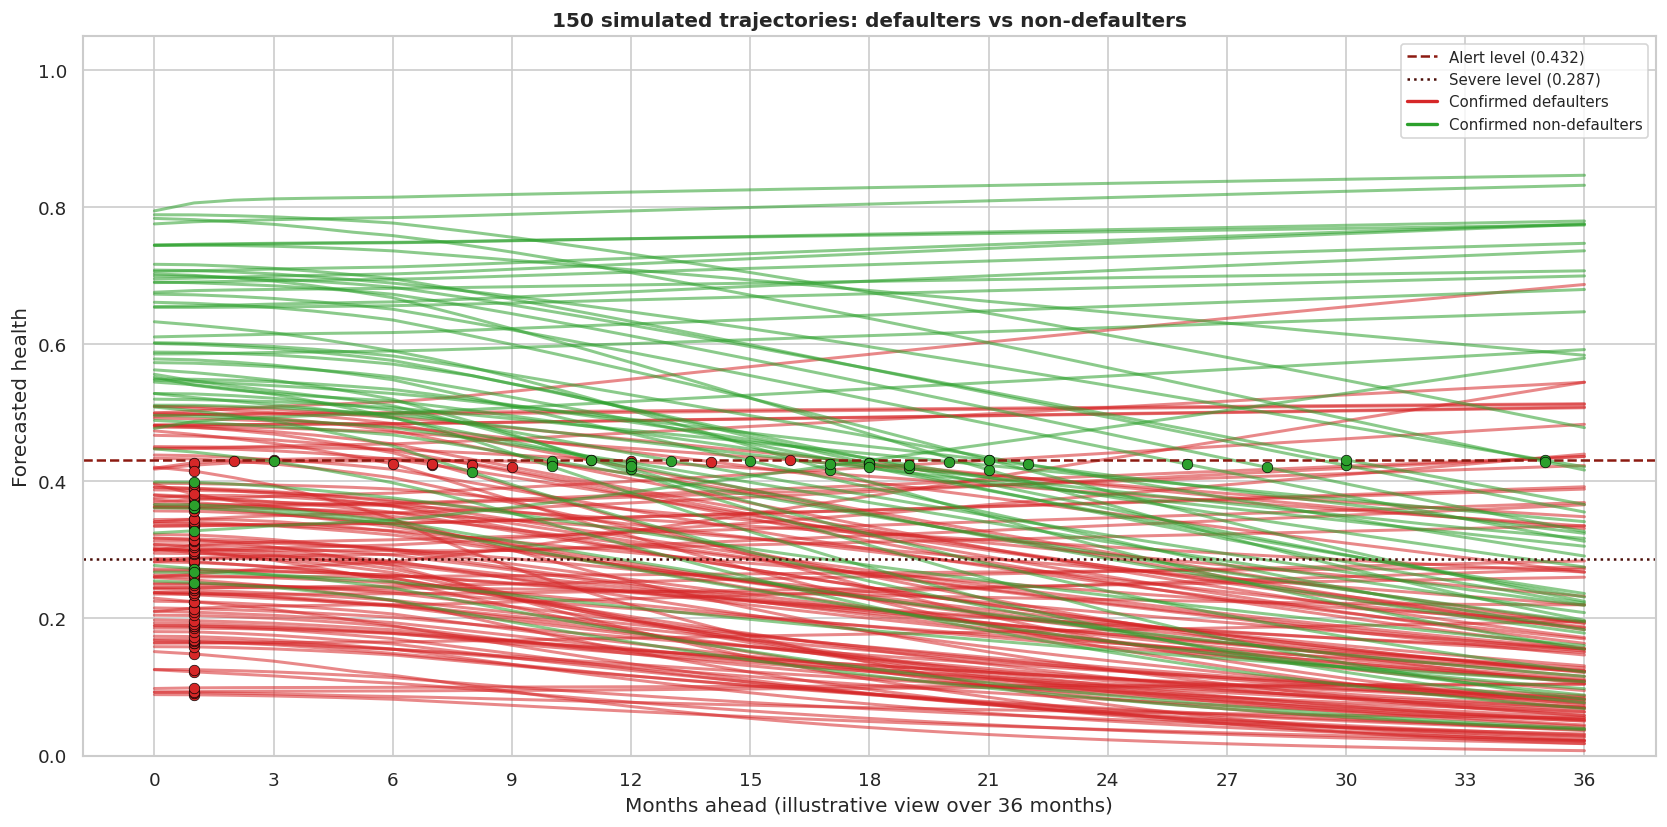
\includegraphics[width=0.98\textwidth]{figures/fig3_simulated_trajectories.png}
\caption{Simulated health trajectories over a 36-month horizon for 150 test borrowers,
coloured by realised outcome. Markers indicate the period at which each trajectory first
crosses the alert threshold. Separation between outcome groups is concentrated in the
early forecast periods, motivating the shortened calibration horizon
(Section~\ref{sec:calibration}).}
\label{fig:traj}
\end{figure}


\subsection{Expected recovery}

An isotonic regression maps forecasted health to expected payment ratio under a
monotonicity constraint, ensuring that higher forecast health cannot imply lower expected
payment. Fit on training data only and multiplied by the outstanding installment amount,
this yields a per-account expected shortfall supporting collections prioritisation prior
to the payment date.

\designnote{Unconstrained regression mapping forecast health to expected payment ratio.}
{An unconstrained fit admits non-monotone regions in which a higher forecast health
implies a lower expected payment. Such regions are artifacts of local sample density
rather than substantive effects, and they are indefensible in a system whose output
informs collections decisions.}
{Isotonic regression, which enforces monotonicity by construction rather than recovering
it incidentally from the data.}

\subsection{Threshold calibration}
\label{sec:calibration}

The system must convert a continuous health forecast into a binary alert decision. The
calibration question is what value that threshold should take, and against what the
threshold should be scored. Three formulations were evaluated.

\subsubsection*{Formulation I: population percentile}

\designnote{Alert threshold set at the 30th percentile of the simulated health
distribution, severe threshold at the 10th.}
{A population percentile mechanically fixes the alert rate. Since non-defaulters
constitute approximately 92\% of the population and therefore dominate the distribution,
``bottom 30\% of the population'' is approximately ``30\% of non-defaulters'' by
construction. The false positive rate was consequently pinned near 30\% irrespective of
any improvement to the underlying model --- the constraint was imposed by the threshold
definition rather than by model performance.}
{Superseded by Formulation III.}

This formulation also produced degenerate thresholds under certain configurations: where
the simulated distribution carried a point mass at a boundary, the 10th and 30th
percentiles resolved to the same value and the two alert tiers collapsed into one.

\subsubsection*{Formulation II: calibrated default probability}

\designnote{$P(\text{default} \mid H)$ estimated by isotonic regression on realised
outcomes, with the threshold set where predicted probability reaches a fixed multiple of
the population base rate.}
{Interpretable and defensible in principle --- the operating point corresponds to a
stated risk appetite (``flag borrowers at least twice as likely to default as
average''). Empirically it did not outperform the ROC formulation, and it introduces an
additional fitted component between the model and the decision, with its own estimation
error.}
{Superseded by Formulation III. The isotonic machinery was retained for the expected
recovery mapping, where a monotone calibrated transform is required.}

\subsubsection*{Formulation III: constrained ROC sweep (retained)}

The retained design abandons any fixed rule and instead searches directly for the
operating point satisfying the stated constraints. The full ROC curve is computed on
training data, and the threshold selected is the one maximising detection subject to the
false-positive budget:
\begin{equation}
\tau^{*} = \arg\max_{\tau} \ \mathrm{TPR}(\tau)
\quad \text{subject to} \quad \mathrm{FPR}(\tau) \leq 0.30
\end{equation}
The selected threshold is then applied to the test set without modification.

This formulation has three properties the earlier designs lack. It corresponds directly
to the stated operating constraints rather than approximating them. It makes
infeasibility explicit --- if no threshold satisfies both constraints, the sweep reports
this rather than silently returning the closest available point, and the required AUC for
feasibility, $(1 + \mathrm{TPR} - \mathrm{FPR})/2$, can be compared against the achieved
AUC to distinguish a threshold problem from a signal problem. And it separates selection
from evaluation cleanly, since the sweep is confined to training data.

\subsubsection*{Scoring quantity}

\designnote{Thresholds scored against terminal simulated health at the forecast horizon.}
{The alert fires the first time a trajectory crosses the threshold, not at the horizon.
Scoring against the endpoint therefore evaluated a different quantity than the alert
logic uses, and a trajectory dipping below the threshold and recovering would be scored
as though it never alerted.}
{Thresholds scored against minimum health reached over the horizon, matching the
first-crossing semantics of the alert.}

\subsubsection*{Forecast horizon}

\designnote{Calibration horizon of twelve months.}
{Trajectory separation between eventual defaulters and non-defaulters is concentrated in
the early forecast periods. Over longer horizons the recursive blend compounds, and the
marginal information in each additional step declines relative to accumulated forecast
variance.}
{Calibration horizon reduced to three months. The thirty-six month simulation is retained
for trajectory visualisation and monitoring tier assignment, where the longer view is
informative, but threshold calibration and alert evaluation operate on the shorter
horizon.}

\subsubsection*{Signal selection}

Several candidate signals are available for the alert decision: the simulated trajectory,
the health score directly, the forecast increment, the external bureau score, and a
direct classifier. Rather than fixing the choice a priori, all candidates are scored on
training data and the strongest is selected, with the selection reported alongside test
performance for each candidate.

\designnote{Candidate signals compared on training AUC, with the direct classifier fit
and scored on the same partition.}
{In-sample scoring necessarily advantages a fitted model over candidate signals not fit
on that data. The classifier reported an AUC of 0.998 and won selection, then generalised
worst of all candidates. The defect corrupted a selection decision rather than a reported
metric, making it invisible in the headline results.}
{Direct classifier scored by out-of-fold prediction under five-fold stratified
cross-validation, placing all candidates on comparable footing.}
\begin{figure}[H]
\centering
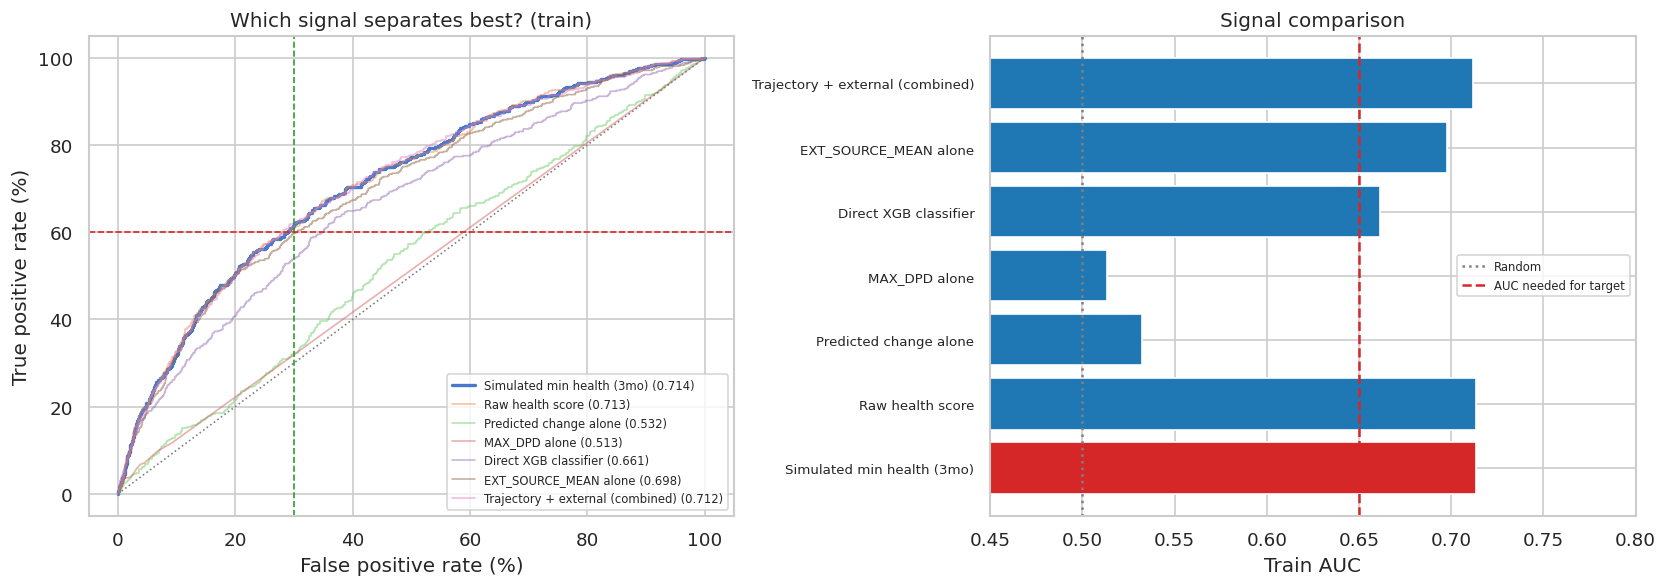
\includegraphics[width=0.98\textwidth]{figures/fig4_signal_bakeoff.png}
\caption{Candidate signal comparison on training data. Left: ROC curves for all candidates,
with the selected signal emphasised; the vertical and horizontal rules mark the
false-positive budget and detection target respectively. Right: AUC by candidate, against
the AUC required for the target operating point to be feasible.}
\label{fig:bakeoff}
\end{figure}


\section{Data Integrity Audit}

The initial pipeline reported $R^2 = 0.985$. A systematic audit identified seven defects,
four constituting information leakage. Corrected, the model reports $R^2 = 0.32$.

\designnote{Model performance accepted on the basis of held-out evaluation alone.}
{A train/test partition detects overfitting but not leakage. Where a feature encodes
information unavailable at prediction time, that information is present in both
partitions, and held-out performance is inflated rather than corrected. An implausibly
strong result on a noisy behavioural forecast is therefore evidence of a construction
defect, not of model quality.}
{Systematic audit of every feature against a single criterion: whether its value at
period $t$ could have been computed using only information available before period $t$.
Each defect below was identified by that test.}

\subsection{Latent stress estimated across full borrower history}

Documented in Section 4.2. An observation at month 5 carried a feature informed by months
6 onward.

\subsection{Mixture models fit prior to partition}

\paragraph{Cause.} Both mixture models were fit before the train/test split, so component
boundaries were informed by test-set borrowers.

\paragraph{Correction.} Borrower-level partition performed first; models fit on training
data and applied to test by transform only. Partition disjointness asserted
programmatically.

\subsection{Acceleration feature reconstructing its target}

\paragraph{Cause.} The feature was constructed as
$\texttt{RAW\_CHANGE}[t] - \texttt{VELOCITY\_LAG1}[t]$, incorporating the current period.
The prediction target was an exponentially-weighted mean (span 2) of that same
$\texttt{RAW\_CHANGE}[t]$, weighting it at approximately 67\%. Therefore
\begin{equation}
\texttt{target}[t] \approx 0.67 \cdot \texttt{ACCELERATION}[t] + \texttt{VELOCITY\_LAG1}[t]
\end{equation}

The model was solving an algebraic identity rather than learning a relationship. The two
features accounted for 55\% of total feature importance.

\paragraph{Correction.} Feature reconstructed from lagged values exclusively. Leading
feature importance subsequently fell to 6.5\%.

\subsection{Contemporaneous features predicting same-period change}
\label{sec:contemporaneous}

\paragraph{Cause.} Features describing period $t$ were the same inputs used to construct
the health score at period $t$, rendering prediction of the change into period $t$
circular. This additionally created a mismatch between training conditions and simulation
conditions, in which only lagged information is available.

\paragraph{Correction.} All snapshot features shifted to prior-period values.

\paragraph{Combined effect of Sections 5.1--5.4.} $R^2$ reduced from 0.985 to 0.32.

\subsection{Cox model misspecification}

\paragraph{Cause.} The model was fit at one observation per borrower-month, each labelled
with the same eventual outcome but a different duration, treating repeated correlated
measurements of a single subject as independent observations. This violates the
independence assumption of the Cox partial likelihood and inflates the effective sample
size.

\paragraph{Correction.} Respecified to one observation per borrower, with durations
derived from observed day-spans rather than binned approximations.

\subsection{Positional rather than temporal lagging}
\label{sec:lagging}

\paragraph{Cause.} Row-position shifts assume an observation in every consecutive period.
A borrower observed at months 3, 4, 7, 8 resolved month 7's prior observation to month 4,
treating a three-month transition as a single-month step.

\paragraph{Correction, first iteration.} Explicit gap validation with velocity normalised
by gap length. This discarded 84\% of observations, since floor-based bucketing against a
global grid misclassifies consecutive payments under real 30.44-day schedules: whether
two genuinely consecutive installments fall one or two buckets apart depends on their
position relative to an arbitrary boundary.

\paragraph{Correction, second iteration.} Bucket boundaries anchored to each borrower's
first installment, with rounding rather than flooring. Observation loss reduced to 56\%;
effective test sample increased from 633 to 1,673 borrowers.

\subsection{In-sample scoring of the baseline classifier}

\paragraph{Observation.} The direct classification baseline reported train AUC 0.998 and
won signal selection, then performed substantially worse on test.

\paragraph{Cause.} The classifier was fit and scored on the same partition. In-sample
scoring necessarily advantages a fitted model over candidate signals not fit on that
data.

\paragraph{Impact.} This defect did not inflate a reported metric. It silently corrupted
a model selection decision, causing the least generalisable candidate to be selected.

\paragraph{Correction.} Out-of-fold prediction under five-fold stratified
cross-validation. The selection procedure is described in Section~\ref{sec:calibration}.

\section{Results}

\subsection{Evaluation design}

\designnote{Alert performance and trajectory validation assessed on subsamples of 100 to
300 borrowers.}
{At an approximate 8\% base rate, a 100-borrower subsample contains roughly eight
defaulters. Detection rates estimated from such a sample carry intervals wide enough to
accommodate most plausible values, and are unstable under reseeding.}
{Evaluation extended to the full test partition. The reported operating point is computed
over 1,673 borrowers containing 138 eventual defaulters.}

\designnote{Model quality reported as AUC alone.}
{AUC summarises ranking across all thresholds and does not indicate whether any single
threshold satisfies a stated operating constraint. Two models with identical AUC can
differ materially at a fixed false-positive budget.}
{Detection rate, false-positive rate, precision and lift reported at the selected
operating point, alongside AUC with interval estimates.}

\subsection{Behavioural score versus commercial bureau score}

\begin{table}[H]
\centering
\caption{Candidate signal performance, behavioural pipeline versus external bureau score}
\begin{tabular}{lccc}
\toprule
\textbf{Signal} & \textbf{Train AUC} & \textbf{Test AUC} & \textbf{95\% CI (test)} \\
\midrule
Raw health score (behavioural) & 0.7134 & 0.7333 & [0.684, 0.782] \\
Trajectory $+$ external combined & 0.7119 & 0.7302 & [0.681, 0.779] \\
Simulated min health (behavioural) & 0.7136 & 0.7300 & [0.681, 0.779] \\
\textbf{Home Credit external bureau score} & 0.6975 & \textbf{0.7220} & [0.672, 0.772] \\
Direct XGBoost (out-of-fold) & 0.6614 & 0.7073 & --- \\
\texttt{MAX\_DPD} alone & 0.5135 & 0.5178 & --- \\
\bottomrule
\end{tabular}
\end{table}

\vspace{6pt}

At a standard error of approximately 0.025 on 138 test defaulters, the behavioural
signals and the bureau score are statistically indistinguishable.

This establishes the principal finding: repayment behaviour observable to a single lender
carries default signal equivalent to a bureau score assembled from a borrower's complete
credit footprint. The mechanism is identifiable in the feature set --- fragmentation,
timing dispersion, and obligation prioritisation are transaction-level signals not
available at bureau level.

\paragraph{Ablation.} Removing \texttt{EXT\_SOURCE\_*} from the direct classifier reduces
performance from 0.707 to 0.612, confirming the external scores carry substantive signal.
The behavioural pipeline achieves 0.730 without dependence on them.

\paragraph{Comparison against unconstrained modelling.} The staged pipeline outperforms a
direct XGBoost classifier on identical features (0.730 versus 0.707), indicating that
decomposition into scoring, forecasting, and simulation stages generalises more
effectively than a single unconstrained model.

\subsection{Operating point}

\begin{table}[H]
\centering
\caption{Test-set operating point against design targets}
\begin{tabular}{lcc}
\toprule
\textbf{Metric} & \textbf{Achieved} & \textbf{Design target} \\
\midrule
Detection rate (TPR) & 64.5\% & $\geq$ 60\% \\
False positive rate & 30.1\% & $<$ 30\% \\
Precision & 16.2\% & base rate 8.2\% \\
Lift over base rate & 1.96$\times$ & --- \\
Test AUC & 0.7300 & train 0.7136 \\
\bottomrule
\end{tabular}
\end{table}

The operating threshold was selected by sweeping the ROC curve on training data for the
constrained operating point, then applied without modification to the test set. Flagged
accounts default at approximately twice the population rate.
\begin{figure}[H]
\centering
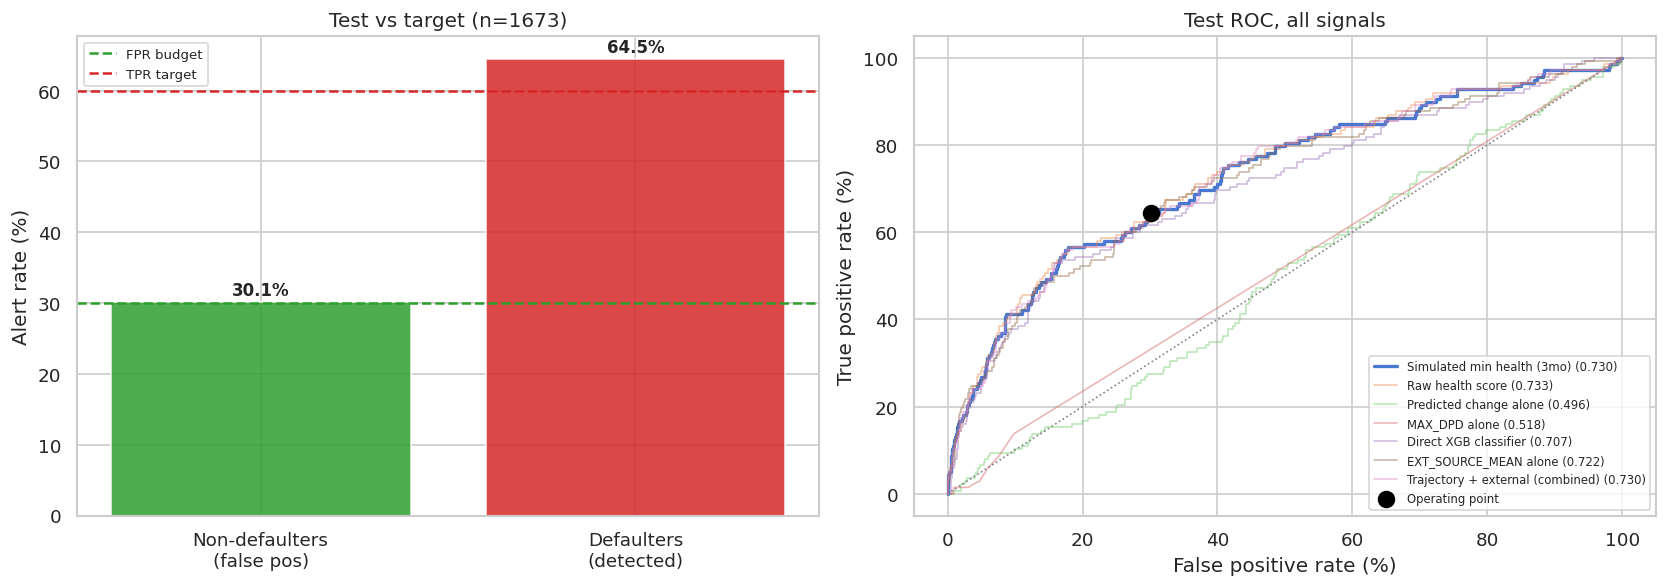
\includegraphics[width=0.98\textwidth]{figures/fig5_test_performance.png}
\caption{Test-set performance. Left: alert rate among eventual defaulters and non-defaulters
against the design targets. Right: test ROC curves for all candidate signals with the
selected operating point marked, overlaid on the corresponding training curve.}
\label{fig:testroc}
\end{figure}


\subsection{Survival validation}

\begin{equation}
\text{C-index} = 0.798
\end{equation}

Specified as one observation per borrower with durations from observed day-spans, the
model confirms the health score as a strong time-to-default predictor, with concordance
approaching 0.80.

\subsection{Operational output}

The simulation layer produces outputs unavailable from a point-in-time score:

\begin{itemize}[leftmargin=1.4em]
\item \textbf{Alert timing} with quantified lead time to threshold crossing
\item \textbf{Monitoring tier assignment} scaling review frequency to forecast risk
\item \textbf{Expected recovery} per account, translating forecast health into an
expected shortfall on the next installment
\end{itemize}
\begin{figure}[H]
\centering
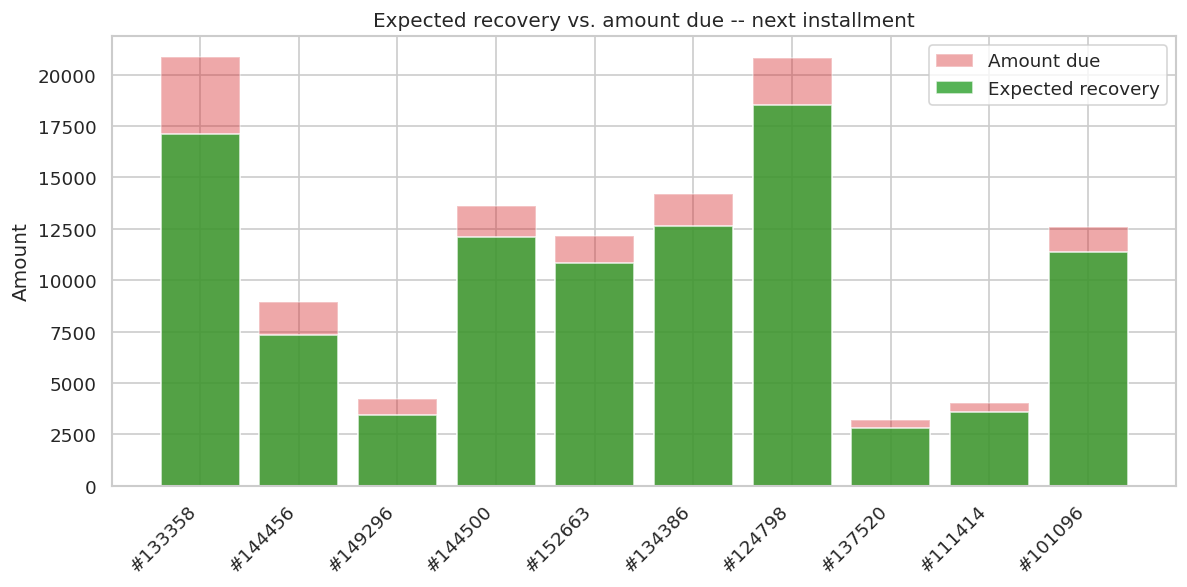
\includegraphics[width=0.86\textwidth]{figures/fig6_expected_recovery.png}
\caption{Expected recovery against amount due for the flagged at-risk batch. The difference
between the two series is the projected shortfall on the next installment, computed prior
to the payment date.}
\label{fig:recovery}
\end{figure}


\section{Conclusions}

A behavioural credit score constructed exclusively from repayment records achieves parity
with a commercial bureau score on held-out borrowers. The result rests on
transaction-level signals --- payment fragmentation, timing dispersion, and obligation
prioritisation --- that are structurally unavailable to bureau-level aggregation.

The staged architecture generalises more effectively than an unconstrained classifier on
identical features, and the survival specification confirms the health score as a strong
time-to-default predictor independently of the classification framing.

The systematic integrity audit is a substantive component of the work. Four leakage
pathways and three methodological defects were identified and corrected, reducing
reported $R^2$ from 0.985 to 0.32 and redistributing feature importance from 55\%
concentration in a single leaked feature to 6.5\% in the leading legitimate feature.

\section{Further Development}

\begin{enumerate}[leftmargin=1.6em]
\item \textbf{Recovery of remaining observation loss.} Calendar-based rather than
fixed-interval bucketing would recover a substantial portion of the 56\% currently
excluded by gap validation, narrowing confidence intervals across all reported results.

\item \textbf{Integration of \texttt{bureau.csv} and \texttt{previous\_\allowbreak application.csv}.}
These sources represent the standard route to higher performance on this dataset and
would permit evaluation against a full-information benchmark rather than external scores
alone.

\item \textbf{Extended observation windows.} Longer per-borrower histories would
strengthen trajectory estimation.

\item \textbf{Cost-weighted threshold selection.} Replacing the constrained operating
point with an explicit cost function over false positives and missed defaults would align
the operating point with realised collections economics.
\end{enumerate}


\section{References}

\begin{enumerate}[label={[\arabic*]},leftmargin=2.4em]

\item Home Credit Group (2018). \textit{Home Credit Default Risk}. Kaggle Competition
Dataset. \texttt{https://www.kaggle.com/c/home-credit-default-risk}

\item Chen, T., \& Guestrin, C. (2016). XGBoost: A Scalable Tree Boosting System.
\textit{Proceedings of the 22nd ACM SIGKDD International Conference on Knowledge
Discovery and Data Mining}, 785--794.

\item Cox, D. R. (1972). Regression Models and Life-Tables. \textit{Journal of the Royal
Statistical Society: Series B}, 34(2), 187--202.

\item Geman, S., \& Geman, D. (1984). Stochastic Relaxation, Gibbs Distributions, and the
Bayesian Restoration of Images. \textit{IEEE Transactions on Pattern Analysis and Machine
Intelligence}, 6(6), 721--741.
\\(Provides the sampling framework underlying the latent stress estimation in Section 4.2.)

\item Dempster, A. P., Laird, N. M., \& Rubin, D. B. (1977). Maximum Likelihood from
Incomplete Data via the EM Algorithm. \textit{Journal of the Royal Statistical Society:
Series B}, 39(1), 1--22.
\\(Standard reference for the mixture-model estimation used in obligation prioritisation.)

\item Si, X.-S., Wang, W., Hu, C.-H., \& Zhou, D.-H. (2011). Remaining Useful Life
Estimation --- A Review on the Statistical Data Driven Approaches. \textit{European
Journal of Operational Research}, 213(1), 1--14.
\\(Source of the degradation-trajectory framing adapted in Section 4.1.)

\item Kaufman, S., Rosset, S., \& Perlich, C. (2011). Leakage in Data Mining:
Formulation, Detection, and Avoidance. \textit{Proceedings of the 17th ACM SIGKDD
International Conference on Knowledge Discovery and Data Mining}, 556--563.
\\(Provides the taxonomy of leakage mechanisms applied in the audit of Section 5.)

\item Barlow, R. E., Bartholomew, D. J., Bremner, J. M., \& Brunk, H. D. (1972).
\textit{Statistical Inference Under Order Restrictions: The Theory and Application of
Isotonic Regression}. Wiley.

\item Hanley, J. A., \& McNeil, B. J. (1982). The Meaning and Use of the Area under a
Receiver Operating Characteristic (ROC) Curve. \textit{Radiology}, 143(1), 29--36.
\\(Basis for the AUC standard-error estimates reported throughout Section 6.)

\end{enumerate}

\end{document}
